\documentclass{article}
\usepackage[utf8]{inputenc}
\usepackage[spanish]{babel}
\usepackage{graphicx}
\usepackage[margin=2.5cm]{geometry}
\usepackage{hyperref}
\usepackage{tikz}
\usepackage{eso-pic}

% --- esto de aquí servirá para poder hacer click en el índice ---
\hypersetup{
    colorlinks=true,
    linkcolor=black,
    urlcolor=blue,
    citecolor=blue
}

\begin{document}

% --- esto de aquí servirá para poner un márgen negro en todas las páginas ---
\AddToShipoutPictureBG{%
    \begin{tikzpicture}[remember picture, overlay]
        \draw[line width=1.5pt, black]
        ([xshift=1cm, yshift=-1cm]current page.north west)
        rectangle
        ([xshift=-1cm, yshift=1cm]current page.south east);
    \end{tikzpicture}%
}

% --- Portada ---
\begin{titlepage}
    \centering

    % --- Encabezado ---
    \begin{minipage}{0.22\textwidth}
        
\includegraphics[width=\linewidth]{Imágenes_Latex/LogoCiencias.png}
    \end{minipage}
    \hfill
    \begin{minipage}{0.52\textwidth}
        \centering
        {\bfseries\Large Universidad Nacional Autónoma de México}\\[0.3cm]
        {\bfseries\large Facultad de Ciencias}
    \end{minipage}%
    \hfill
    \begin{minipage}{0.22\textwidth}
        
\includegraphics[width=\linewidth]{Imágenes_Latex/UNAM_Logo.png}
    \end{minipage}%

    \vspace{0.4cm}
    \rule{\textwidth}{1pt}
    \vspace{2.5cm}

    % --- Título del proyecto ---
    {\Huge \bfseries Proyecto Chat} \\[0.5cm]
    {\Large Cliente y Servidor para un Chat} \\[2.5cm]

    % -- Datos ---
    \rule{0.8\textwidth}{0.5pt}\\[0.5cm]

    \begin{large}
        \textbf{Autor:} Fernando Chablé Alonzo \\
        \textbf{Profesor:} Canek Peláez Valdéz \\
        \textbf{Ayudantes:} Cynthia Lizbeth Sánchez Urbano y Miriam Torres Bucio \\
        \textbf{Asignatura:} Modelado y Programación \\
        \textbf{Fecha:} \today
    \end{large}

    \rule{0.8\textwidth}{0.5pt}\\[0.5cm]

    \vfill

\end{titlepage}

% Numeración de las páginas
\clearpage
\pagenumbering{arabic}

% -- Índice ---
\tableofcontents
\clearpage

% --- Contenido ---

% --- Resumen ---
\section{Resumen}
En este reporte se presenta el diseño e implementación de un sistema de chat concurrente basado en la arquitectura cliente-servidor.

El sistema se fundamenta en el uso de sockets TCP y la gestión de hilos de ejecución (threads) para garantizar una comunicación fluida,
ordenada y simultánea entre múltiples clientes.
Para la construcción del proyecto, el servidor fue desarrollado en lenguaje C haciendo uso
de las librería \texttt{cJSON} para un control eficiente de memoria, mientras que el cliente se estructuró en C\# mediante el SDK de
.NET. La arquitectura modular sigue el patrón Modelo-Vista-Controlador (MVC) y cumple con un protocolo de comunicación de doce comandos que
abarca la identificación de usuarios, mensajería pública y privada, y la administración dinámica de salas apoyada en listas ligadas simples.

Finalmente, se discuten los aprendizajes adquiridos, las dificultades técnicas durante la implementación en red y las posibles líneas de trabajo
futuro.

\vspace{2cm}
(No se me ocurre más resumen xd).

\clearpage

% --- Introducción ---
\section{Introducción}
Este proyecto contiene algunos conceptos medianamente complejos, tales como \textbf{sockets TCP}, \textbf{concurrencia}, \textbf{hilos de ejecución},
entre algunos otros por lo que veo necesario explicarlos brevemente a continuación:

\subsection{¿Qué es la arquitectura Cliente Servidor?} \cite{arqui_cliente_servidor}
La \textbf{arquitectura Cliente Servidor} podemos definirla como un modelo de diseño de software en el cual las aplicaciones se dividen el trabajo entre
dos componentes principales: \textbf{clientes} y \textbf{servidores}. Esta separación facilita la gestión de recursos y hace que ambos interactúen de manera
eficiente, pues el cliente se dedica a realizar solicitudes de \textit{servicios} o \textit{datos} al servidor, y el servidor se dedica a proporcionar esos
\textit{recursos} que requiere el cliente.

\begin{figure}[htbp]
    \centering
    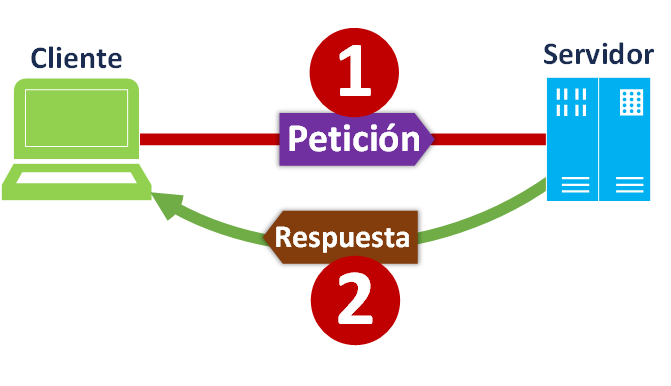
\includegraphics[width=0.6\textwidth]{Imágenes_Latex/Cliente-y-servidor.png}
    \caption{Diagrama de la arquitectura cliente-servidor. Fuente: \cite{cliente_servidor_jarroba}}
\end{figure}

En el caso de este proyecto, el \textbf{servidor} se encarga de escuchar todas solicitudes de los diferentes \textbf{clientes}, sean solicitudes para \textit{identificarse},
\textit{mandar mensajes}, \textit{crear salas}, entre otras. El \textbf{cliente} le manda una solicitud al \textbf{servidor} con datos que proporcionó el usuario, el
\textbf{servidor} procesa esos datos y le responde al \textbf{cliente} (o incluso a los demás clientes) su solicitud para que el usuario los vea.

\subsection{¿Qué son los sockets TCP?} \cite{sockets_tcp}
Un \textbf{socket} lo podemos definir como un punto final de comunicación entre dos programas o dispositivos, son los responsables de conectar esos mismos dos programas o
dispositivos. Los \textbf{sockets} siguen dos protocolos diferentes: \textbf{TCP} y \textbf{UDP}, y en el caso de este proyecto se usaron \textbf{sockets TCP}.
El protocolo \textbf{TCP} es un protocolo de la capa de transporte que está orientado a \textbf{conexión}, por lo que antes de intercambiar datos debe haber un paso
para poder establecer una comunicación. Además, \textbf{TCP} garantiza que la información llegue en correcto estado, pues si la información tarda en llegar o llega
dañada, el propio \textbf{TCP} se encarga de volverla a mandar, y una última ventaja que tienen es que los datos que manda se envían en \textbf{orden}.

\subsection{¿Qué es la concurrencia?} \cite{concurrencia}
La \textbf{concurrencia} podemos definirla como la \textbf{ejecución simultanea} de múltiples procesos, esto permite que diferentes partes de un programa funcionen
de manera independiente, lo que eficientiza el uso de recursos y la experiencia del usuario. Dentro de la \textbf{concurrencia} tenemos otro concepto importante, que son
los \textbf{hilos de ejecución}.

\subsubsection{¿Qué son los hilos de ejecución/threads?}
Los \textbf{hilos de ejecución} (mejor conocidos como \textbf{threads}) son por así decirlo caminos de ejecución pequeños dentro de un proceso. En un entorno concurrente,
muchos \textbf{hilos de ejecución} pueden coexistir, donde cada uno tiene una tarea específica.

\begin{figure}[htbp]
    \centering
    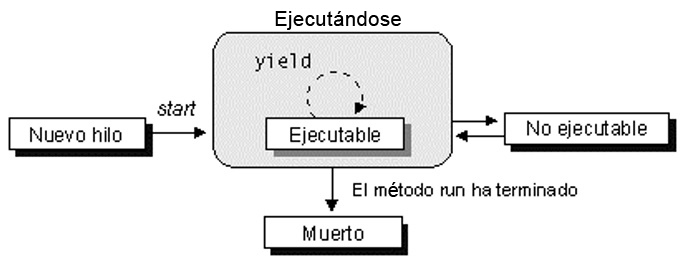
\includegraphics[width=0.6\textwidth]{Imágenes_Latex/threads.jpg}
    \caption{Diagrama de un hilo de ejecución. Fuente: \cite{hilos_ejecucion}}
\end{figure}

\subsection{¿Qué es un protocolo?}
Por último, un \textbf{protocolo de comunicación} podemos definirlo como las reglas o el formato que tanto el \textbf{cliente} como el \textbf{servidor} siguen par
entenderse sin que se presente ninguna ambigüedad o algo parecido. (Sí, no hay mucho que decir de qué es un protocolo hasta donde yo sé).

\clearpage

% --- Análisis y diseño ---
\section{Análisis y diseño}
En esta sección vamos a ver (de manera un poco breve) el análisis que hice sobre nuestro problema y el diseño de la solución que hice. En este caso, nuestro problema era
hacer un chat usando la arquitectura Cliente Servidor, que fuera concurrente y, lo más importante, \textbf{FUNCIONAL}.

\subsection{Análisis}
Pude deducir rápidamente que el problema sí era computable, pues si dividimos el problema en diferentes subproblemas nos darémos cuenta que sí se pueden hacer en un número finito de pasos, más considerando que la cantidad de usuarios que se conectarán al servidor son
finitos, por lo que (mientras esté bien hecho), todos esos subproblemas tendrán un fin.
Los diferentes subproblemas en los que lo dividí son:

\begin{itemize}
    \item \textbf{Servidor}
        \begin{itemize}
        \item Crear y manejar los hilos de ejecución para cada usuario.
        \item Crear un socket para poder escuchar y aceptar conexiones entrantes.
        \item Procesar y responder los datos que mande cada usuario.
    \end{itemize}
    \item \textbf{Cliente}
        \begin{itemize}
        \item Crear un socket para poder conectarse al servidor.
        \item Procesar y mandar los datos del usuario al servidor.
    \end{itemize}
\end{itemize}

Además, gracias al protocolo que nos proporcionó el profesor, ya teníamos otra parte del problema (todo lo que constituía al chat) dividida en más subproblemas:

\begin{itemize}
    \item IDENTIFY: El usuario se identifica con un username único. Si no se identifica no puede hacer nada.
    \item STATUS: El usuario cambia su estado actual a otro.
    \item USERS: Se le muestra al usuario una lista con todos los usuarios conectados.
    \item TEXT: El usuario manda un texto privado a otro.
    \item PUBLIC TEXT: El usuario manda un texto público.
    \item NEW ROOM: El usuario crea una nueva sala.
    \item INVITE: El usuario invita a más usuarios a una sala.
    \item JOIN ROOM: El usuario se une a una sala en la que fue invitado.
    \item ROOM USERS: Se le muestra al usuario una lista con los usuarios de una sala.
    \item ROOM TEXT: El usuario manda un mensaje a una sala.
    \item LEAVE ROOM: El usuario sale de una sala.
    \item DISCONNECT: El usuario se desconecta del chat.
\end{itemize}

Y sí, como ya se pudo dar cuenta querido lector, el chat también tendrá \textbf{salas} (como los grupos de WhatsApp o los servidores de Discord).

\subsection{Diseño}
Tuve que definir unas cuántas estructuras para poder manejar a los \textit{usuarios} y a las \textit{salas}, y a su vez definí dos listas para
poder manejar a todos los \textit{usuarios} y a todas las \textit{salas}.

\begin{itemize}
    \item \textbf{ClienteNodo}:
    \begin{itemize}
        \item \textit{Atributos}:
        \begin{itemize}
            \item Socket (un entero que represente al socket del usuario).
            \item Username (un string que represente el username del usuario).
            \item Status (un string que represente el estado actual del usuario).
            \item Siguiente (un puntero que apunte a otro ClienteNodo que represente al usuario que sigue del actual).
        \end{itemize}
    \end{itemize}

    \item \textbf{ListaClientes}:
    \begin{itemize}
        \item \textit{Atributos}:
        \begin{itemize}
            \item Cabeza (un puntero que apunte a un ClienteNodo que está en la lista y que representa a la cabeza de la misma).
            \item NumClientes (un entero que represente a la cantidad de usuarios que hay en la lista).
        \end{itemize}
        \item \textit{Métodos}:
        \begin{itemize}
            \item \texttt{crear\_lista}: Inicializa una lista de clientes desde cero.
            \item \texttt{insertar\_cliente}: Crea un nuevo cliente con los datos proporcionados y lo mete a la lista.
            \item \texttt{eliminar\_cliente}: Elimina a un cliente de la lista basándose en el socket proporcionado.
            \item \texttt{buscar\_cliente}: Revisa si un cliente existe en la lista.
            \item \texttt{limpiar\_lista}: Se encarga de limpiar la memoria usada por la lista.
        \end{itemize}
    \end{itemize}

    \item \textbf{NodoSala}:
    \begin{itemize}
        \item \textit{Atributos}:
        \begin{itemize}
            \item Room\_name (un string que represente el nombre de la sala).
            \item Usuarios (un puntero que apunta a una ListaClientes que almacena a los usuarios de la sala).
            \item Invitados (un puntero que apunta a otra ListaClientes que almacena a los usuarios que se han invitado a la sala).
            \item Siguiente (un puntero que apunta a un NodoSala que represente a la sala que sigue de la actual).
        \end{itemize}
    \end{itemize}

    \item \textbf{ListaSalas}:
    \begin{itemize}
        \item \textit{Atributos}:
        \begin{itemize}
            \item Cabeza (un puntero que apunta a un NodoSala que está en la lista y que representa a la cabeza de la misma).
            \item Num\_salas (un entero que represente a la cantidad de salas que hay en la lista).
        \end{itemize}
        \item \textit{Métodos}:
        \begin{itemize}
            \item \texttt{crear\_lista\_salas}: Inicializa una lista de salas desde cero.
            \item \texttt{insertar\_sala}: Crea una nueva sala con el nombre proporcionado y lo mete a la lista.
            \item \texttt{eliminar\_sala}: Elimina una sala de la lista basándose en el nombre proporcionado.
            \item \texttt{buscar\_sala}: Revisa si una sala existe en la lista.
            \item \texttt{obtener\_sala}: Obtiene la dirección de la sala en la lista y del nombre proporcionado.
            \item \texttt{limpiar\_lista\_salas}: Se encarga de limpiar la memoria usada por la lista.
        \end{itemize}
    \end{itemize}
\end{itemize}

Como se puede ver, elegí implementar listas ligadas simples para poder almacenar a los usuarios y las salas, esto porque me parecen bastante
fáciles de implementar y eficientes, pues tienen un tamaño dinámico y son fáciles de manejar.

El protocolo proporcionado por el profesor incluye \textbf{doce métodos}, métodos que salen en el \textbf{análisis}, y para explicar cómo los
diseñé usaré diagramas secuenciales en UML, pero para no inundar el reporte con doce diagramas, los voy a resumir a tres.

\clearpage

\begin{figure}
    \centering
    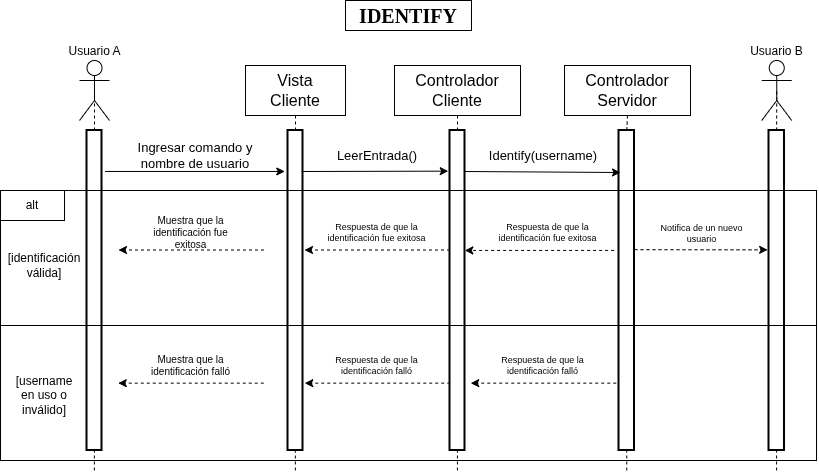
\includegraphics[width=1\textwidth]{Imágenes_Latex/Diagrama_Identify.png}
    \caption{Diagrama UML de IDENTIFY.}
\end{figure}

\begin{figure}
    \centering
    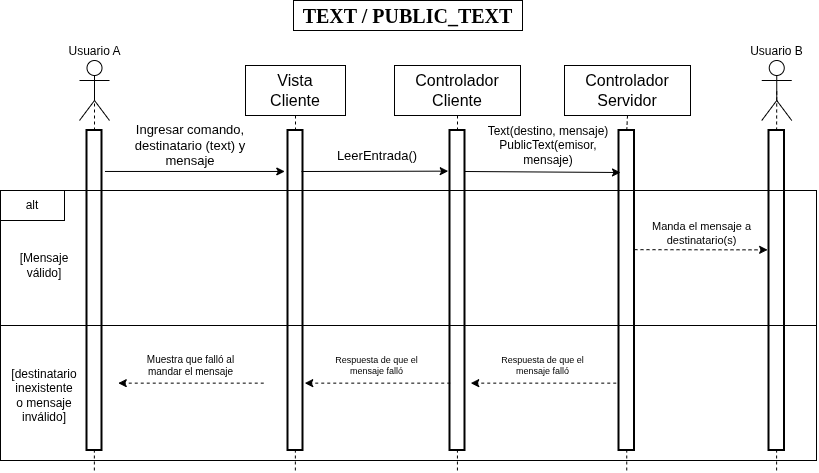
\includegraphics[width=1\textwidth]{Imágenes_Latex/Diagrama_Text_PublicText.drawio.png}
    \caption{Diagrama UML de TEXT y PUBLIC\_TEXT.}
\end{figure}

\clearpage

\begin{figure}
    \centering
    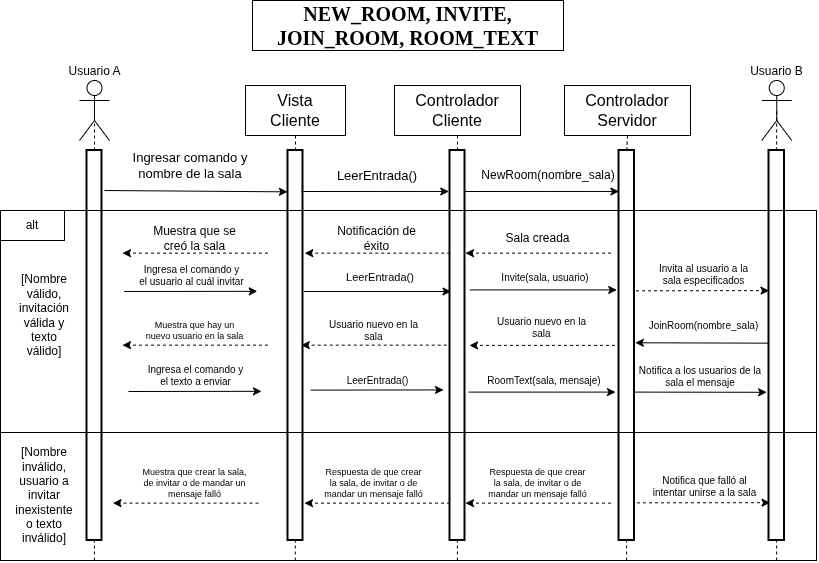
\includegraphics[width=1\textwidth]{Imágenes_Latex/Diagrama_de_salas.png}
    \caption{Diagrama UML de NEW\_ROOM, INVITE, JOIN\_ROOM y ROOM\_TEXT.}
\end{figure}

No veo necesario hacer los diagramas UML de los demás métodos pues me parecen demasiado sencillos y saturarán de información el reporte.

Sinceramente no se me ocurre una mejor manera para poder implementar estos métodos, pues estas implementaciones cubren prácticamente todos
los casos posibles y tienen una respuesta para cada uno.

\clearpage

% --- Implementación ---
\section{Implementación}
Para poder implementar el diseño que hice, usé dos lenguajes de programación: \textbf{C} para hacer el servidor y \textbf{C\#} para hacer el
cliente. Usé \textbf{C} para el servidor pues me daba curiosidad aprender este lenguaje, más considerando los punteros, y por eso mismo me
parece un lenguaje bastante eficiente (siempre y cuando manejes bien la memoria, claro); y usé \textbf{C\#} para el cliente pues era el lenguaje
del que más tenía conocimiento (después de Java, pero ese no lo podíamos usar).

Los únicos requerimentos para poder compilar y ejecutar el servidor y el cliente son los siguientes:
\begin{itemize}
    \item \textbf{Servidor}:
    \begin{itemize}
        \item Para poder compilar el servidor se necesita tener instalado el compilador \textbf{GCC} (hasta donde sé, todas las
        distribuciones de Linux ya lo tienen por default), realmente no se necesita algo más, solo tendrías que ubicarte en la carpeta de nombre
        \textbf{servidor}, y ejecutar el siguiente comando: \textbf{gcc -Wall main.c modelo/ListaClientes.c modelo/ListaSalas.c vista/red\_vista.c
        controlador/chat\_controlador.c -lcjson -lpthread -o servidor}
        Luego, para poder ejecutar el servidor, solamente tienes que escribir \textbf{./servidor} en la carpeta donde se creó el ejecutable.
    \end{itemize}
    \item \textbf{Cliente}:
    \begin{itemize}
        \item Para poder compilar el cliente se necesita tener instalado el \textbf{SDK} de \textbf{.NET}, pues contiene el compilador de C\#,
        el runtime de .NET y las librerías base de C\#. Para compilar y ejecutar el cliente, tendrías que ubicarte en la carpeta de nombre
        \textbf{ClienteChat} y ejecutar el siguiente comando: \textbf{dotnet run}, con ese simple comando se compila todo el proyecto de C\#
        y lo ejecuta automáticamente.
    \end{itemize}
\end{itemize}

\clearpage

% --- Conclusiones ---
\section{Conclusiones}
Me parece que las conclusiones las puedo dividir en varias secciones.

\subsection{¿Qué aprendí?}
En lo personal yo aprendí a manejar sockets, a construir un servidor y un cliente usando la arquitectura cliente servidor, a manejar varios casos
que pueden hacer los usuarios, a poder dividir un proyecto así de grande (sé que no es grande pero es el más grande que he hecho hasta la fecha)
usando el patrón MVC, a poder seguir un protocolo sin perderme en el intento, y a usar mejor C y C\#.

\subsection{¿Qué se me dificultó?}
Pienso que lo más difícil fue entender el cómo hacer el servidor, cómo hacer el cliente y cómo hacer que se comuniquen, esto porque no tenía
absolutamente nada de conocimiento sobre sockets ni de las librerías que los implementan en C y C\#. A su vez, tampoco sabía nada sobre la
arquitectura cliente servidor, y tampoco sobre hilos de ejecución, por lo que aprender de estos concepctos fue lo que más me robó tiempo
considerando que es de lo más rápido (porque obviamente implementar el protocolo fue lo que más me robo tiempo, pero eso fue por ser muy
tardado).

\subsection{¿Qué pude mejorar?}
Sobre todo creo que puedo mejorar en cómo estructuro mi código, pues en algunos métodos se repiten las mismas ocho líneas de código, cosa que
se podía solucionar haciendo un método auxiliar con esas ocho líneas, además que tanto código puede llegar a abrumar al que lo intenta comprender
a falta de comentarios. Otra cosa que también pude haber mejorado es haber implementado una interfáz gráfica, pues es mucho más intuitivo usar
la interfáz gráfica de un programa que usar comandos en la terminal.

\subsection{Si quisiera expandir el sistema, ¿Qué propondría?}
En mi caso, yo propondría que el chat tenga soporte para mandar diferentes archivos, sean archivos de texto, de audio, imágenes, etc. Además, no
estaría mal poner alguna clase de filtro en el chat, pues como está hecho ahorita cualquier cosa (incluyendo ilícitas) pueden expresarse en el chat.
Y por último, intentaría hacer que el IDENTIFY sea un poco más estricto, y en vez de identificarte solo con el nombre, te tengas que identificar
con tu nombre y alguna contraseña que hayas hecho antes (para evitar robos de identidad o algo parecido).

\clearpage

% --- Bibliografía ---
\section{Bibliografía}

\begin{thebibliography}{99}

    % Arquitectura Cliente-Servidor
    \bibitem{arqui_cliente_servidor}
    Gomez, C. (2024). \textit{Qué es la arquitectura cliente servidor y cómo funciona}. \url{https://www.daemon4.com/empresa/noticias/arquitectura-cliente-servidor/}

    % Imagen Cliente-Servidor
    \bibitem{cliente_servidor_jarroba}
    Invarato, R. (2019). \textit{Cliente vs Servidor}. \url{https://jarroba.com/cliente-vs-servidor/}

    % Sockets TCP
    \bibitem{sockets_tcp}
    De Luz, S. (2025). \textit{Qué es un socket TCP o UDP y qué diferencias hay con los puertos}. \url{https://www.redeszone.net/tutoriales/configuracion-puertos/que-es-socket-tcp-udp-diferencias-puertos/}

    % Concurrencia e hilos de ejecución
    \bibitem{concurrencia}
    Lenovo (s/f). \textit{¿Qué es la concurrencia?}. \url{https://www.lenovo.com/mx/es/glosario/concurrencia/}

    % Imagen hilos de ejecución
    \bibitem{hilos_ejecucion}
    UNAM (s/f). \textit{Hilos}. \url{https://repositorio-uapa.cuaed.unam.mx/repositorio/moodle/pluginfile.php/3084/mod_resource/content/1/UAPA-Hilos/index.html}

\end{thebibliography}

\end{document}